\documentclass[manuscript,review,anonymous]{acmart}
\usepackage{caption}
\usepackage{subcaption}
\usepackage{hyperref}

% NOTE: Good things
%  - what is iterative prompting? "Like auto-complete but less limited" - hmm, maybe
%  - sell more main idea: can do much with very limited set of commands / via auto-complete
%  - paper is convincing in that this works for SQL-like queries (maybe not general purpose, but this is good)
%  - journalism is a good focus / but needs to deemphasize this a bit because of the study
%  - #1 Limited language for data exploration (what is included / excluded / essential / could be added)
%  - #2 Iterative prompting - what's new? people can get to all programs via '.' and up/down/enter.

% NOTE: Random
%  - How choices were made?
%  - Terminology: data analysis / data exploration / data visualization - what is the goal of the system? (fair enough)
%    (it's not about writing charts - just about getting the right data - we have limited charting functionality,
%     one could integrate with Vega, or do future work based on iterative prompting)
%  - Technical details - you can only create valid programs!! (it's contextual)
%  - Minor: what was "demo" at the start of a session
%  - Table 1 vs. Table 2 numbers of participants
%  - What data quality is needed to make this work?
%  - "Magic Escalator of Knowledge" - remove bs?
%  - Clarify how we support 3D cubes (no unified API); mention "done by intern in X weeks"

% TODO
%   - SAY SOMEWHERE: choose function *and* specify arguments via auto-complete
%   - ADD: table of all available operations? (shorten introduction)

% NOTE: Contribution
%  - What is the exact goal? (so that it can be compared with R, Python, Vega-Lite, Tableau)
%  - How the design goals were generated? (not by talking to journalists)
%  - "notebooks are messy" - not arguing we can fix that

% NOTE: Motivation
% - what if you could write the whole program using auto-complete?

% Explain type providers a bit more (we say what it does, but not much about what
% it is - give dynamic typing in a static language)
%
% The 'then' operation was mysterious - can we add one line explanation to the operations?
% (yes we can and we should totally do that)




% \usepackage{xspace}
\usepackage{fancyvrb}
% \usepackage{inconsolata}
\usepackage{xcolor}
\usepackage{tikz}
\newcommand*{\priority}[1]{\begin{tikzpicture}[scale=0.12]%
   \draw (0,0) circle (1);
   \fill[fill opacity=1,fill=black] (0,0) -- (90:1) arc (90:90-#1*3.6:1) -- cycle;
   \end{tikzpicture}}
\newcommand*{\priorityc}[1]{
\resizebox{0.8em}{0.8em}{
 {\protect\tikz{ \protect
   \draw[line width=1mm, black] (0,0) circle (1); \fill[fill opacity=1,fill=black] (0,0) -- (90:1) arc (90:90-#1*3.6:1) -- cycle;
   } }}}
%
\definecolor{kvdclr}{rgb}{0.3,0.0,0.8}
\DefineVerbatimEnvironment{thegamma}{Verbatim}{fontfamily=zi4,numbers=left,xleftmargin=6mm,fontsize=\small,commandchars=\\\{\}}
% %\newcommand{\kvd}[1]{\textcolor{kvdclr}{#1}}
\newcommand{\kvd}[1]{\textbf{#1}}
\newcommand{\ikvd}[1]{{\fontfamily{zi4}\selectfont\small #1}}
% \usepackage{balance}       % to better equalize the last page
% \usepackage{graphics}      % for EPS, load graphicx instead
% \usepackage[T1]{fontenc}   % for umlauts and other diaeresis
% \usepackage{txfonts}
% \usepackage{mathptmx}
% \usepackage[pdflang={en-US},pdftex]{hyperref}
% \usepackage{color}
% \usepackage{booktabs}
% \usepackage{textcomp}

\setcopyright{acmwhatever}
\copyrightyear{2020}
\acmYear{2020}
%\acmDOI{10.1145/1122445.1122456}
\acmConference[Woodstock '18]{Woodstock '18: ACM Symposium on Neural
  Gaze Detection}{June 03--05, 2018}{Woodstock, NY}
\acmBooktitle{Woodstock '18: ACM Symposium on Neural Gaze Detection,
  June 03--05, 2018, Woodstock, NY}
\acmPrice{15.00}
%\acmISBN{978-1-4503-XXXX-X/18/06}

\begin{document}
\title{The Gamma: Data Exploration through Iterative Prompting}

\author{Tomas Petricek}
\email{t.petricek@kent.ac.uk}
\affiliation{%
  \institution{University of Kent}
  \city{Canterbury, UK}
}
%\renewcommand{\shortauthors}{Trovato and Tobin, et al.}

\begin{abstract}
  Governments, non-profit organizations and citizen initiatives publish increasing amounts of
  data, but extracting insights from such data and presenting them to the public is hard.
  First, data comes in a variety of formats that each requires a different tool. Second, many
  data exploration tools do not reveal how a result was obtained, making it difficult to reproduce
  the results and check how they were obtained.
  %
  We contribute The Gamma, a novel data exploration environment for non-experts. The Gamma is based
  on a single interaction principle and using it results in transparent and reproducible scripts.
  This allows transfer of knowledge from one data source to another and
  learning from previously created data analyses. We evaluate the usability and learnability of
  The Gamma through a user study on non-technical employees of a research institute.
  %
  We argue that our approach allows journalists and the public to benefit from the rise
  of open data, by making data exploration easier, more transparent and more reproducible.

\end{abstract}

\begin{CCSXML}
<ccs2012>
   <concept>
       <concept_id>10003120.10003121.10003124</concept_id>
       <concept_desc>Human-centered computing~Interaction paradigms</concept_desc>
       <concept_significance>500</concept_significance>
       </concept>
   <concept>
       <concept_id>10011007.10011006.10011050.10011017</concept_id>
       <concept_desc>Software and its engineering~Domain specific languages</concept_desc>
       <concept_significance>300</concept_significance>
       </concept>
   <concept>
       <concept_id>10011007.10011006.10011066.10011069</concept_id>
       <concept_desc>Software and its engineering~Integrated and visual development environments</concept_desc>
       <concept_significance>500</concept_significance>
       </concept>
 </ccs2012>
\end{CCSXML}

\ccsdesc[500]{Human-centered computing~Interaction paradigms}
\ccsdesc[500]{Software and its engineering~Integrated and visual development environments}
\ccsdesc[300]{Software and its engineering~Domain specific languages}
\keywords{data exploration; end-user programming; data journalism; programming languages; type providers}

\maketitle

\begin{figure}
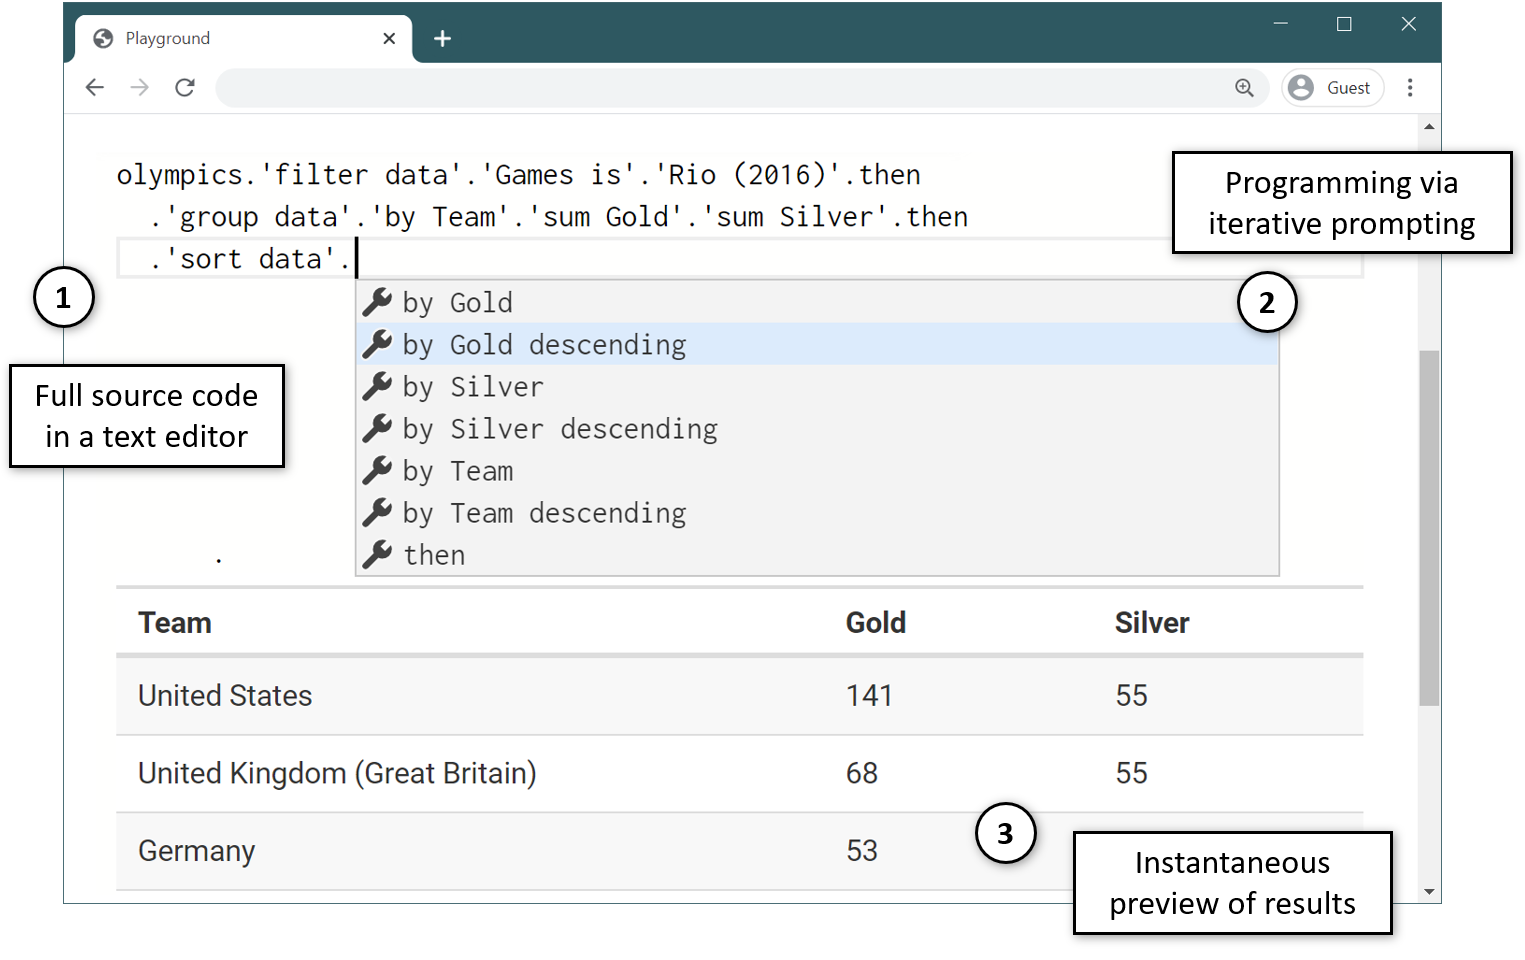
\includegraphics[width=.58\columnwidth]{figures/thegamma-annot}
\vspace{-0.5em}
\caption{Obtaining teams with the greatest number of gold medals from Rio 2016
Olympics with a reproducible The Gamma script (1), contextual iterative prompting mechainsm
offering ways of sorting the data (2) and an instant preview of results (3).}
\label{fig:thegamma}
\vspace{-0.5em}
\end{figure}

% ==================================================================================================

\section{Introduction}
Data science has more capabilities to help us understand the world than ever before, yet at the
same time post-truth politics and increasing public distrust in statistics makes data-driven insights
increasingly less relevant in public discourse~\cite{howstatslost}. To reverse this trend, we
need tools that let non-experts, including journalists and other information-literate citizens,
produce transparent, engaging data analyses that are easy to interpret without requiring expert
programming skill~\cite{ddj}. The design of such data exploration tool poses a unique mix of chellenges.
First, the tool needs to have a very low barrier to entry. Second, it needs to support a wide
range of data sources in a uniform way. Third, the resulting data analyses need to assist
readers in learning how to reproduce the work and verify the claims it makes.

We contribute The Gamma, a text-based data exploration environment for non-experts. The Gamma
is based on a single, easy to understand interaction principle and provides a uniform
access to a range of data sources including data tables, graph databases and data cubes.
The resulting analysis is a transparent script that can be followed to reproduce the
result from scratch. This allows learning from existing analyses and encourages readers
to engage with data.

\subsubsection*{Iterative Prompting}
The key idea in The Gamma, which we term the \emph{iterative prompting} principle, is that all
valid data exploration scripts can be constructed by repeatedly choosing from a list
of offered options. This way, non-programmers can write entire scripts through auto-complete,
without learning a programming language, but they still produce transparent and reproducible
source code. In other words, iterative prompting turns auto-complete from a programmer assistance
tool into a non-expert programming mechanism. A crucial feature is that iterative prompting
only offer operations that are valid in a given context and that it offer all such operations;
it is both correct and complete.

\subsubsection*{Data Exploration}
The Gamma focuses on data exploration of the kind illustrated in Figure~\ref{fig:thegamma}.
The user accesses data available in a structured format. They make several experiments to find an
interesting way of looking at the data, e.g.~by applying different aggregations or filters. They
may choose to view the results as a table or a basic chart before publishing their analysis. The
Gamma makes such simple programming with data simple enough for non-experts. Scraping and cleaning
of messy data or building rich data visualizations is outside of the scope of this paper, but
exposing those using the iterative prompting approach is an interesting future challenge.

\subsubsection*{Contributions}
The Gamma is available (non-anonymously) at \url{http://thegamma.net},
both as a JavaScript library and a hosted data exploration service. In this paper, we describe and
evaluate the design principles behind the project:

\begin{itemize}
\item We introduce the iterative prompting principle in The Gamma
  and show that it can be used for querying of distinct data sources including data tables, graph
  databases and data cubes (Section~\ref{sec:overview}).

\item We reflect how our design addresses challenges faced by journalists (Section~\ref{sec:design-ddj})
  and analyse the design theoretically. We argue that our design lowers barriers to entry (Section~\ref{sec:design-bar}),
  supports learning without experts (Section~\ref{sec:design-expert}) and offers a
  complete and correct program construction method (Section~\ref{sec:design-cc}).

\item We evaluate the system through a number of case studies (Section~\ref{sec:cases})
  and a user study (Section~\ref{sec:study}). Our study shows that non-programmers can use The Gamma
  to construct non-trivial data queries and ascertains the extent to which users can,
  (i) learn from examples and (ii)~transfer knowledge between tasks.
\end{itemize}

% ==================================================================================================

\section{Related Work}

The key contribution of our work is that it develops a new, fundamentally different, way of using the
established auto-completion mechanism. Unlike most past work dating back to Kaiser~\cite{assistants},
we do not view it as a programmer assistance tool, but as an interaction mechanism through which
non-experts can create entire programs. We build on recent research on information-rich
programming \cite{inforich} and aim to make those advances available to non-programmers
\cite{enduser,smallmatter}, in the context of data exploration as done, most notably, by
journalists \cite{ddj}. Our work features a novel combination of characteristics in that
the iterative prompting we develop (i) is centered around editing and understanding of program code,
(ii) its conceptual complexity is reduced to a single basic kind of interaction, yet (iii) it is
correct and complete in that it can be used to construct all meaningful programs.

\subsubsection*{Code Completion for Data Science}

A key component in The Gamma is the use of auto-complete for offering possible operations.
Our work follows type providers \cite{inforich,fsdata}, which integrate external data into a
static type system of F\#, allowing the use of auto-completion; for querying data tables, we utilize
the theory developed by Petricek \cite{dotdriven}. The key difference in our work is that The Gamma
can be used without a programming language expertise.

Most similar to our approach are tools that recommend scripts when users begin interacting
with data. Those based on machine learning code completion for domain specific languages \cite{predictive,proactive}
differ in that they do not guarantee completeness, i.e.~the user cannot create all possible
scripts. Approaches based on natural language can effectively support data exploration
or visualization \cite{eviza,codemend}, but hide the structure of the underlying language and
require more than just selecting options. Conversational agents \cite{iris} improve on such work
in that they can provide more guidance. Code completion based on machine learning or statistical
methods \cite{mlcomplete,statcomplete} also exists for general-purpose programming languages used
by data scientists such as Python \cite{pythia}, providing assistance to expert programmers.
Finally, DS.js \cite{dsjs} is interesting in that it enables querying of data on the
web; it uses JavaScript with rich contextual code completion.

\subsubsection*{Notebooks and Business Intelligence Tools}

Notebooks such as Jupyter \cite{jupyter}, which allow combining source code with commentary and
visual outputs, are widely used by data scientists, but require expert programming skills.
The Gamma targets non-experts, but could be easily integrated with a multi-language notebook system
such as Wrattler \cite{wrattler}.

Spreadsheets and business intelligence tools \cite{tableau,powerbi} do
not involve programming, but require mastering a complex GUI. This is also the case
for other visual data analytics tools \cite{control,vizdom}. In contrast, The Gamma is
based on a single kind of interaction. Several visual systems \cite{potter,wrangler,lyra} record
interactions with the GUI as a script that can be seen and modified by the user.
Unlike in The Gamma, the source code does not guide the user in learning how to use the system.

\subsubsection*{Easier Programming Tools}
We aim to build an easy to use and learn programming system. Many approaches to this
goal have been tried. Victor \cite{principle} introduced design principles that
inspired many to build live programming systems \cite{review,liveroad,lighttable} that give
immediate feedback to help programmers understand how code relates to output and
exploratory systems \cite{variolite,exploratory} that assist with completing open-ended tasks.
A system combining textual language with visualization also exists for graph querying \cite{guess}.
To avoid difficulties with editing code as text, some systems use structured editors~\cite{structure-based,livenut,lamdu}.
In Subtext \cite{subtext,directprog} the language itself is co-designed with the editor to make
the interactions with code more natural. The Gamma is live in that our editor gives an instant
preview of the results.

Many systems simplify programming by designing high-level declarative abstractions,
e.g.~for interactive news articles \cite{idyll}, statistical analyses \cite{tea}
or interactive data visualization \cite{interactionviz,vegalite}. The Gamma uses
high-level abstractions for data querying, but designing high-level iterative prompting
abstractions for other tasks remains future work.

\subsubsection*{Programming without Writing Code}
There are two main approaches to programming where
the user does not write code. In programming by example \cite{byexample}, the user gives
examples of desired results. This has been used, e.g.~for specifying data transformations
in spreadsheets and data extraction \cite{spreadsheetpbe,flashextract}.
In direct manipulation \cite{direct}, a program is specified by directly interacting with the
output. This has been used in the visual domain \cite{sketchnsketch}, but also for data querying
\cite{dynamicq,vlang}. The VQE language~\cite{visage} also considers how to allow code reuse and
modification in this context. Direct manipulation can also support data exploration by letting
users partially edit queries,~e.g. by changing quantifiers as in DataPlay~\cite{dataplay}.

\subsubsection*{Guestures and Data Entry}
Although our focus is on program construction, our work can be positioned in the
broader context of input methods. Akin to Dasher \cite{dasher}, our system provides a way of
navigating through a complete space of options, while on-screen feedforward \cite{octopocus} allows
efficient selection in guesture-based interfaces. Those provide compelling alternatives to
auto-completion menus, although the efficiency of input methods is not an issue in programming.


\begin{figure}[b]
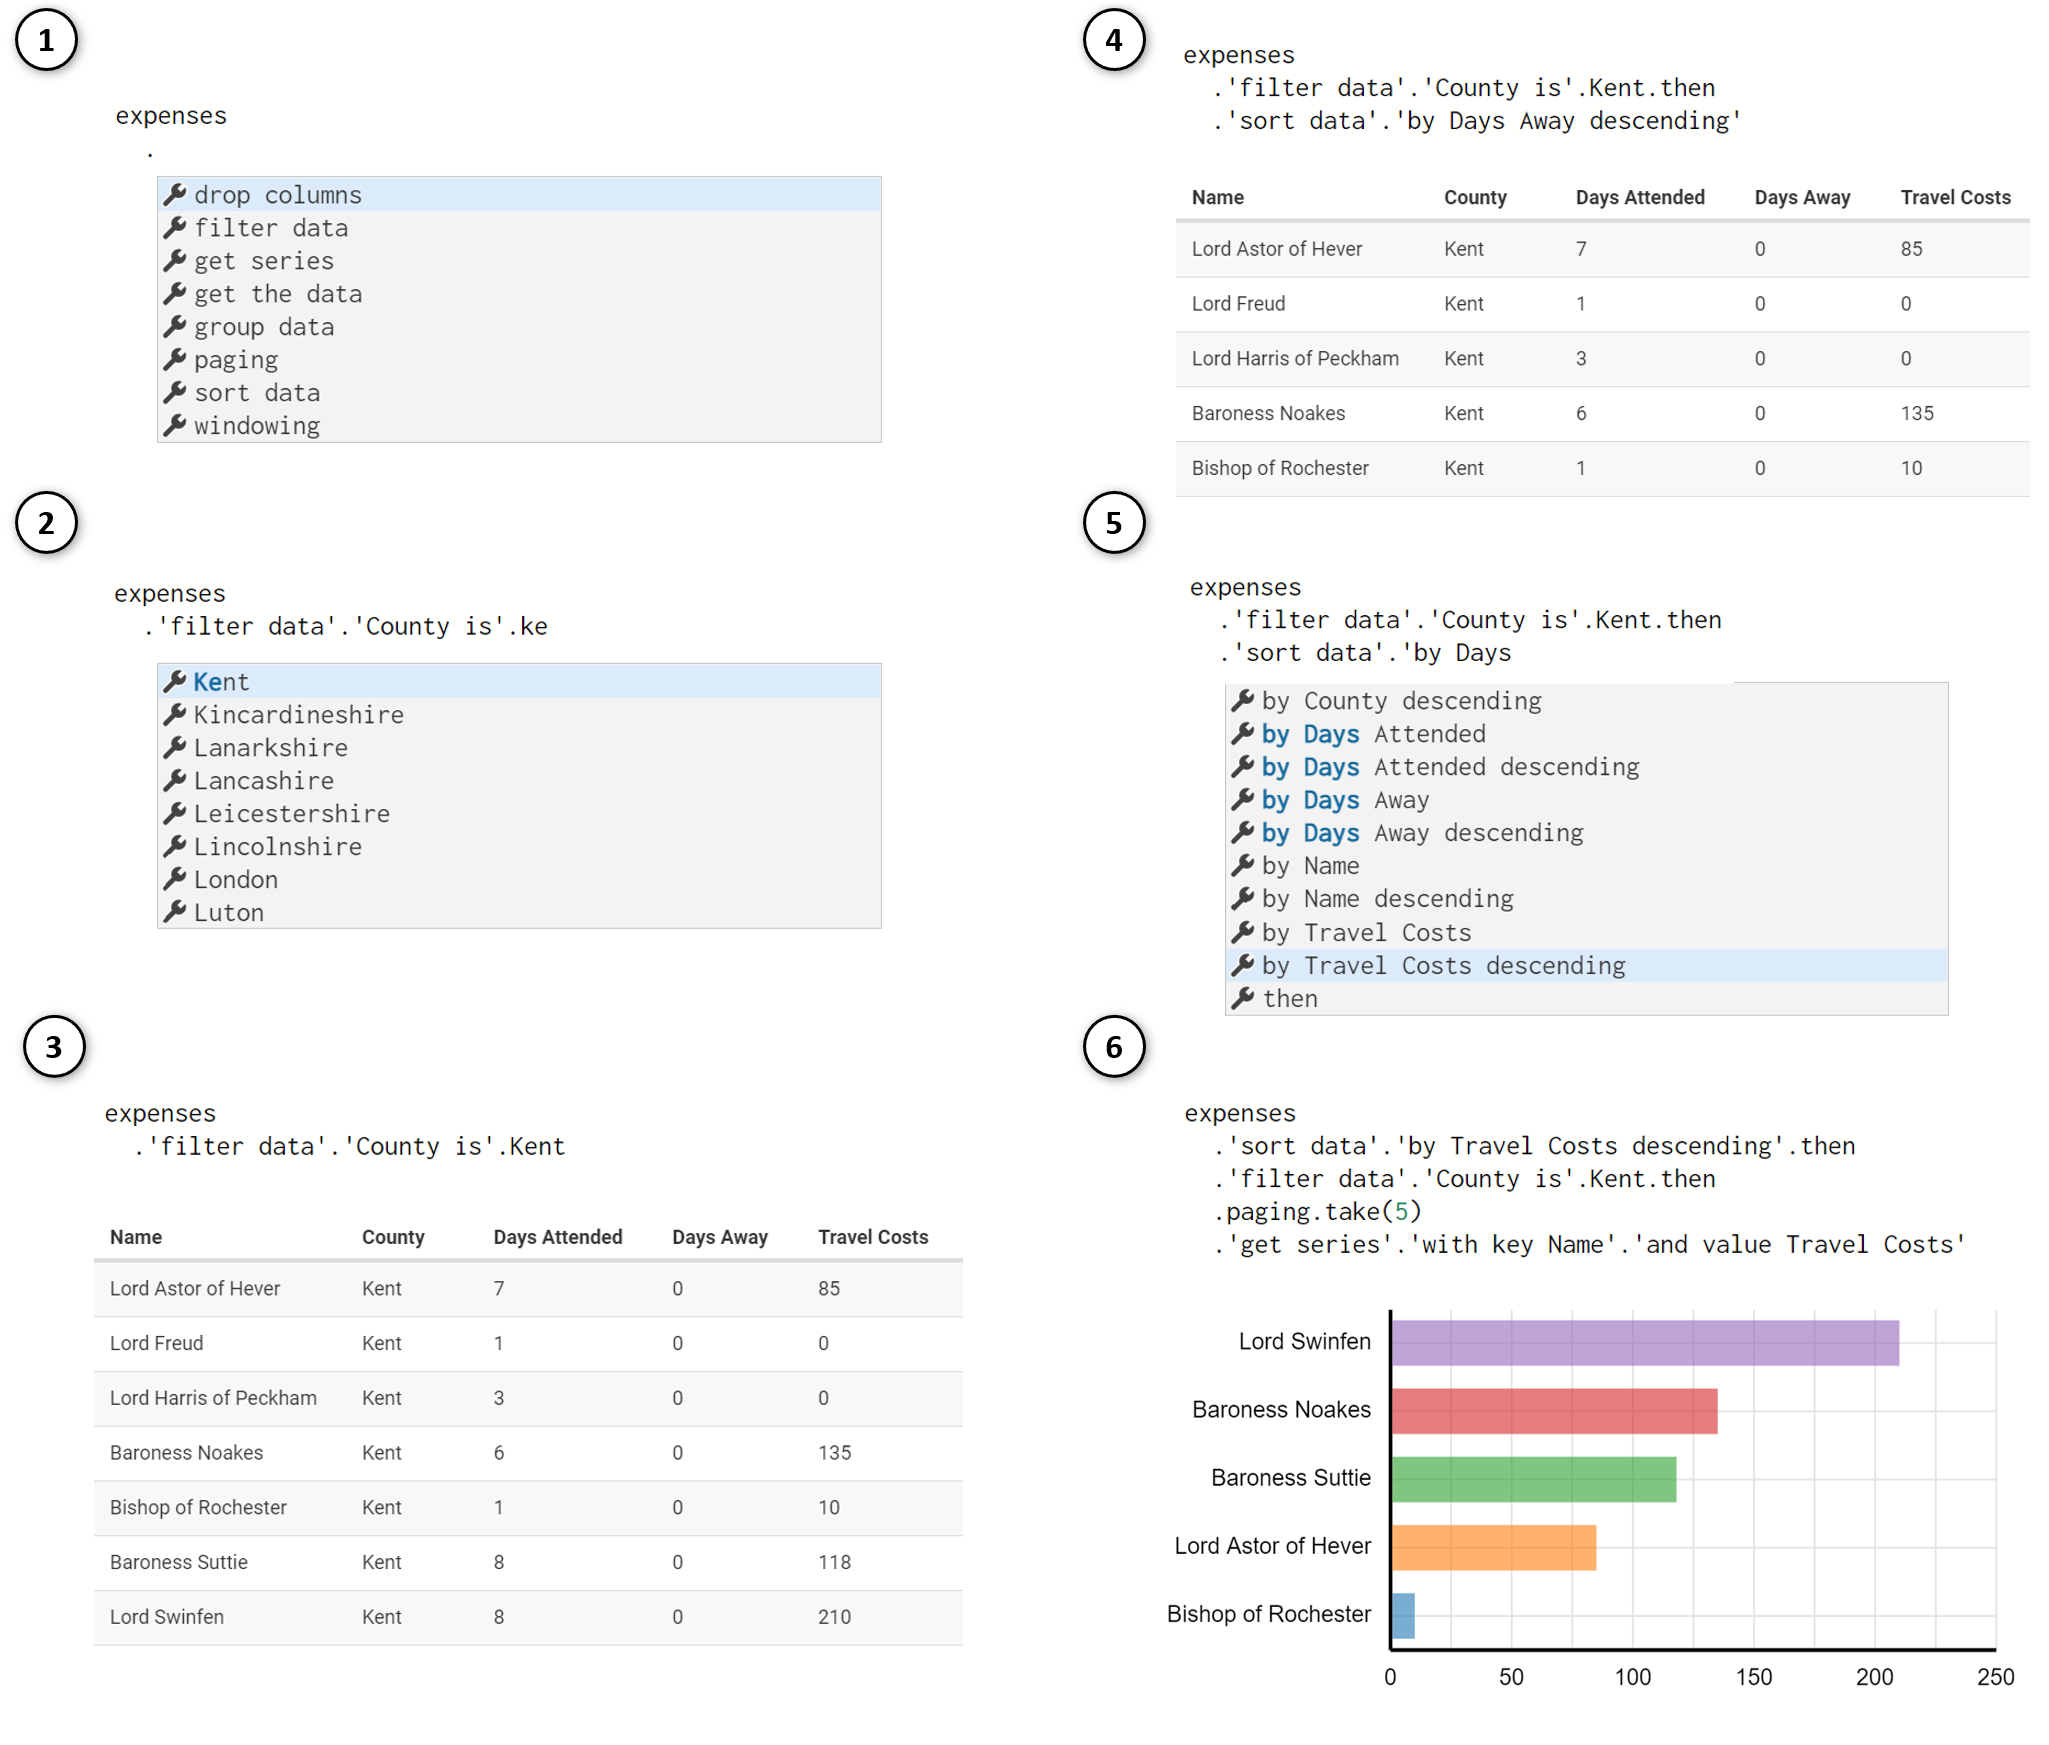
\includegraphics[width=1\columnwidth]{figures/thegamma-walk}
\caption{Constructing a script that charts the top 5 members of the House of Lords for Kent, based
on their travel costs.}
\label{fig:walkthrough}
\end{figure}

% ==================================================================================================

\section{Overview}
\label{sec:overview}

The review of related work suggests that there is an unexplored point in the design space of tools
for data exploration. Although various efforts make text-based programming easier, e.g. by providing
high-level declarative abstractions, most systems that target non-experts shy away from code, by using
either programming by example, natural language or graphical user interface. As spelled out in
Section~\ref{sec:design}, text-based programming has notable benefits for public-facing data analyses
such as learnability and transparency. Our work is thus motivated primarily by the question whether we
can make text-based programming easy enough for non-experts? The study presented in Section~\ref{sec:study}
shows that this is, indeed, possible at least for typical data querying tasks.
The Gamma consists of a programming language, a web-based coding environment and a number of type providers
that enable access to various kinds of data sources. It allows non-experts to create programs using the
\emph{iterative prompting} interaction principle -- by repeately selecting an item from an auto-complete list.
We start with a walkthrough of the system (Section~\ref{sec:overview-walk}), before looking at details of
The Gamma language (Section~\ref{sec:overview-lang}) and individual type providers (Section~\ref{sec:overview-tps}).

\subsection{Querying Travel Expenses}
\label{sec:overview-walk}

To introduce The Gamma, we walk through a simple problem that a local journalist might want to solve.
The UK government publishes travel expense claims by members of the House of Lords. We want to find
out which of the members representing the Kent county spend the most on travel.
The following shows a subset of the data:\footnote{Full data set has been obtained from
\url{https://www.parliament.uk/mps-lords-and-offices/members-allowances/house-of-lords/holallowances/} }

\begin{thegamma}
\textbf{Name, County, Days Attended, Days Away, Travel Costs}
Lord Adonis, London, 8, 0, 504
Baroness Afshar, Yorkshire, 2, 0, 0
Lord Alderdice, Oxfordshire, 3, 0, 114
Lord Alli, London, 5, 0, 0
\end{thegamma}
% Baroness Amos, London, 3, 0, 0

\noindent
The data is available as a CSV file. After the analyst imports the file through a web interface,
the environment is initialized with code that refers to the imported data as \ikvd{expenses}
and she starts exploring the data using the type provider for tabular data (Section~\ref{sec:overview-tps}),
following the steps illustrated in Figure~\ref{fig:walkthrough}:

\begin{enumerate}
\item The analyst types `.' (dot) to trigger auto-completion on \ikvd{expenses}. The type provider
  offers a list of operations that the analyst might want to perform such as grouping,
  filtering and sorting.

\item To find the House of Lords with the largest spending, the analyst chooses the
  \ikvd{sort data} operation. Next, she is offered a list of possible arguments based on the
  schema of the tabular data and chooses the desired one.

\item The Gamma evaluates the source code on-the-fly and shows a preview
  of results. After choosing the sorting key, the analyst sees a table with House of Lords members
  from more remote counties of the UK.

\item To finish specifying the (possibly compound) sorting key, the analyst chooses \ikvd{then}
  and is offered the same list of querying operations as in the first step. To obtain House
  members from Kent, she chooses \ikvd{filter data}. To navigate through the offered list more
  efficiently, she types first two characters of the name.

\item After selecting \ikvd{County is} to specify the desired type of condition, the analyst types
  `.' and is offered a list of options based on the values of the \ikvd{County} column in the
  source data set. She types \ikvd{Ke} and selects \ikvd{Kent}.

\item The analyst chooses \ikvd{then} and is,
  again, offered the list of querying operation. She uses \ikvd{paging} to get top 5 records,
  which requires typing \ikvd{5} as the argument. She then uses the \ikvd{get series} operation
  to obtain a data series associating travel expenses with a name, which is automatically
  visualized using a bar chart.
\end{enumerate}

\noindent
The constructed code is not unlike an SQL query, except that the whole script is constructed using
iterative prompting, by repeatedly selecting one of the offered members. Those represent both
operations, such as \ikvd{sort by} and arguments, such as \ikvd{Kent}. The only exception
is when the analyst needs to type the number \ikvd{5} to specify the number of items to take.

\subsection{The Gamma Programming Environment}
\label{sec:overview-lang}

The Gamma consists of a text-based programming language with a web-based coding environment,
based on the Monaco editor\footnote{For more information, see \url{https://microsoft.github.io/monaco-editor/}},
and type providers that provide access to data tables, graph databases and data cubes.

\subsubsection*{The Gamma Language}
A program in The Gamma is a sequence of commands. A command can be either a variable declaration
or an expression that evaluates to a value such as a data table or a chart.
An expression is a reference to a data source followed by a chain of member accesses.
A member can be either an ordinary member such as \ikvd{paging} or an operation which takes a
list of parameters enclosed in parentheses as in \ikvd{take(5)}. When the member name contains
non-alphanumerical characters it is  written in quotes such as \ikvd{\textquotesingle sort by\textquotesingle}.

The Gamma uses a type system to infer what members are available at a given point in a chain.
Each expression has a type with a list of members that, in turn, have their own types.
The types are not built-in, but are generated by type providers for individual data sources.
The programming environment for The Gamma is based on a text editor. When the user types `.'
the editor triggers auto-completion and retrives a list of available members based on the type
information. The programming environment evaluates scripts on-the-fly and shows a preview as
illustrated in Figure~\ref{fig:thegamma}.

\subsubsection*{Making Complex Things Possible}
As illustrated by the \ikvd{take(5)} operation, there is a handful of situations where The
Gamma does not yet fully support the iterative prompting principle. The language supports
a small number of other features that can be used by more advanced users through text editing:

\vspace{0.3em}
\begin{thegamma}
\kvd{let} topTravel = expenses.'sort data'.'by Travel Costs descending'.then
  .paging.take(5).'get series'.'with key Name'.'and value Travel Costs'
charts.column(topTravel).setColors(["red","blue","green"])
  .setTitle("House of Lords members by travel expenses")
\end{thegamma}
\vspace{0.3em}

\noindent
First, The Gamma allows operations with parameters such as \ikvd{take(5)} or \ikvd{setTitle("...")}.
This is currently needed when writing a query that skips or takes first N elements from a table.
The remaining features are not needed for basic data exploration. The \ikvd{let} construct can be
used to define (immutable) variables and The Gamma also supports lists written as \ikvd{[1,2,3]}.
Advanced language features are currently used when building custom charts, but we expect that a
charting library compatible with iterative prompting would alleviate the need for most of those.


\subsection{Type Providers for Data Querying}
\label{sec:overview-tps}

The Gamma can be extended to support any kind of data source by implementing a \emph{type provider}.
Conceptually, a type provider defines a domain specific language for exploring data of a particular
kind. Techincally, it generates object types with members (such as \ikvd{sort by} or \ikvd{Count is})
that are accessed via iterative prompting. We describe type provider for exploring data cubes
(inspired by an example from Syme et al. \cite{inforich}), tabular data (based on theory developed
by Petricek \cite{dotdriven}), and a novel type provider for exploring graph databases.

\subsubsection*{Data Cube Type Provider}
Our first type provider allows users to explore data form a data cube. For example, the World
Bank\footnote{The data is retrived using an API available at: \url{https://data.worldbank.org/}}
collects a range of indicators about many countries in the world each year. The data set is a
three-dimensional cube with dimensions corresponding to countries, indicators and years. The
following example uses the provider to access CO$_{2}$ emission data for United States:

\begin{thegamma}
worldbank.byCountry.'United States'.'Climate Change'.'CO2 emissions (kt)'
\end{thegamma}

\noindent
As illustrated in Figure~\ref{fig:cubetp}, the provider allows users to select a data series
from the data cube. Choosing \ikvd{byCountry.\textquotesingle United States\textquotesingle},
restricts the cube to a two-dimensional plane. We then choose an indicator category
and a specific indicator \ikvd{\textquotesingle CO2 emissions (kt)\textquotesingle}, obtaining
a time series with years as keys and emission data as values. Similarly, we could first filter the
data by a year or an indicator. The same mechanism can be used for exploring the UK government
expenditure:

\begin{thegamma}
expenditure.byService.Defence.inTermsOf.GDP
\end{thegamma}

\noindent
The dimensions of the cube are government services, years and value type (adjusted, nominal,
per GDP). Here, we select the \ikvd{Defence} service and \ikvd{GDP} value type.
As there is no widely used standard format for data cubes, adding another data cube to The Gamma
currently requires implementing a new type provider.

\subsubsection*{Tabular Data Type Provider}

Our second type provider allows users to construct queries to explore data in tabular formats
such as CSV files. A prominent example of tabular data used by journalists is, e.g.~the
Iraq War documents leak~\cite{iraq}. Unlike the data cube provider, the provider for tabular data does not just
allow selecting a subset of the data, but it can be used to construct SQL-like query. Consider
the example from Figure~\ref{fig:thegamma}:

\begin{thegamma}
olympics.'filter data'.'Games is'.'Rio (2016)'.then
  .'group data'.'by Team'.'sum Gold'.'sum Silver'.then
  .'sort data'.'by Gold descending'
\end{thegamma}

\noindent
The example works with a CSV file that records individual medals awarded in Olympic games.
The chain constructs a query that selects rows corresponding to the Rio 2016 Olympics and then
calculates total number of gold and silver medals for each team (country) before sorting the data.

When using the provider, the user specifies a sequence of operations. Members such as
\ikvd{\textquotesingle filter data\textquotesingle} or \ikvd{\textquotesingle group data\textquotesingle}
determine the operation type. Those are followed by operation parameters. For example, when grouping
data, we first select the key and then choose a number of aggregations to calculate over the group.
Unlike SQL, the provider only allows users to choose from pre-defined aggregations such as
calculating the sum, average or the number of distinct values. As illustrated in
Section~\ref{sec:cases}, this is sufficient to construct a wide range of practical queries.


\begin{figure}
\centering
\begin{subfigure}[b]{0.5\textwidth}
  \centering
  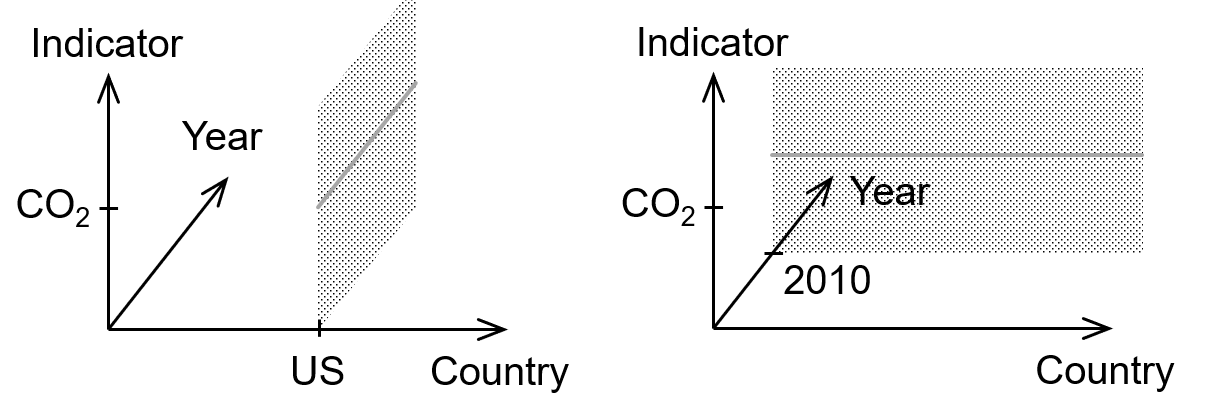
\includegraphics[scale=0.25]{figures/cubetp}
  \vspace{0.5em}
  \caption{Exploring World Bank data using the data cube type provider, users
    choose values from two dimensions to obtain a data series.}
  \label{fig:cubetp}
\end{subfigure}
\hfill
\begin{subfigure}[b]{0.45\textwidth}
  \centering
  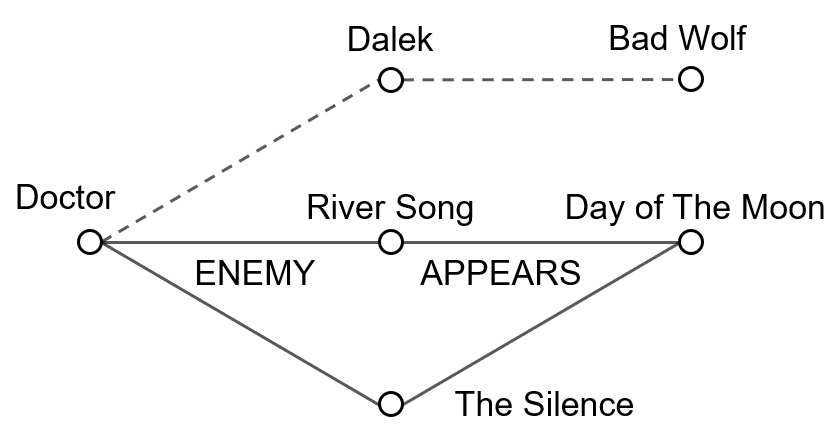
\includegraphics[scale=0.28]{figures/graphtp}
  \caption{To query graph data, the user specifies a path through the data, possibly with
    placeholders to select multiple nodes.}
  \label{fig:graphtp}
\end{subfigure}
\vspace{-0.5em}
\caption{Design of type providers for exploring data cubes and graph databases.}
\label{fig:tps}
\end{figure}


\subsubsection*{Graph Database Type Provider}
Our third type provider allows users to explore data from graph databases, which store
nodes representing entities and relationships between them. In the context of data journalism,
graph databases have been used for example in The Panama Papers reporting \cite{panama}.
The following example explores a database of Doctor Who characters and episodes. It retrieves
all enemies of the Doctor that appear in the Day of the Moon episode:

\begin{thegamma}
drwho.Character.Doctor
  .'ENEMY OF'.'[any]'.'APPEARED IN'.'Day of the Moon'
\end{thegamma}

\noindent
We start from the \ikvd{Doctor} node and then follow two relationships. We use
\ikvd{\textquotesingle ENEMY OF\textquotesingle.\textquotesingle [any]\textquotesingle}
to follow links to all enemies of the Doctor and then specify
\ikvd{\textquotesingle APPEARED IN\textquotesingle.\textquotesingle Day of the Moon\textquotesingle}
to select only enemies that appear in a specific episode. The resulting query
is illustrated in Figure~\ref{fig:graphtp}.

The provider works with any graph database and generates members automatically, based on the
data in the database. In the above example, \ikvd{ENEMY OF} and \ikvd{APPEARED IN} are labels
of relations and \ikvd{Doctor} and \ikvd{Day of the Moon} are labels of nodes. The
\ikvd{[any]} member defines a placeholder that can be filled with any node with the specified
relationships. The results returned by the provider is a table of properties of all nodes
along the specified path. As illustrated by an example discussed in Section~\ref{sec:cases},
the returned table can be further queried using the tabular data type provider.

% ==================================================================================================

\section{Reflections on Design}
\label{sec:design}

The design of The Gamma has been motivated by a curiosity as to whether iterative
prompting can make text-based programming with data accessible to non-experts. In this section,
we theoretically assess the resulting design and position it in the context of a possible application
in the context of data journalism.

\subsection{Data Journalism Perspective}
\label{sec:design-ddj}

Although our work targets non-expert data exploration in general, data journalism is an important
specific domain with interesting design requirements. We reflect those on the basis of relevant
literature, e.g.~\cite{ddj,edcj17,edcj18} and past experience of collaborating with
journalists. Two challenges faced by journalists \cite{future} are particularly relevant to The Gamma.

\subsubsection*{Trust Through Transparency}
The first issue is trust in media. Many practitioners believe that transparency
about the editorial process and information sources can serve as a proof of quality and
trustworthiness~\cite{transparency}. This applies to data analyses too. For example, the Financial Times
increasingly share source code of their analyses on GitHub, e.g.~\cite{ftnotebooks},
but reproducing such analyses is difficult even for an expert. The Gamma has a potential to
improve on the status quo in that a part of the analysis can be directly embedded in an article.
The source code provides full account of what the data sources are and how are they used.
The Gamma makes this code, to a greater extent, accessible to non-expert readers.

\subsubsection*{Encouraging Meaningful Engagement}

The second challenge is developing relationship with readers. Journalists are looking
for meaningful ways of engagement through reader comments, involvement of citizen journalists
\cite{comments,citizen} and the development of new interactive formats \cite{youdraw}.
The Gamma can support this aim by providing a data exploration environment that can engage
non-expert readers in a meaningful discussion. As argued below, non-experts can learn to use the
system and can, for example, modify parameters or change filtering criteria to get a
new perspective on a story.

\subsection{Lowering Barriers to Entry}
\label{sec:design-bar}

Data exploration has a certain irreducible essential complexity. To make it accessible to users who
cannot dedicate much time to learning a tool prior to using it, this complexity needs to be
carefully stratified. The Gamma uses a two-level structure. At the first level, the user needs
to learn iterative prompting to be able to start exploring data. At the second level, users will
need to learn domain specific languages defined by individual type providers.

\subsubsection*{Iterative Prompting Principle}
Iterative prompting is a suitable first level principle, because it is easy to trigger.
In conventional programming languages, auto-complete assistance is only available once basic
code structure is written. In contrast, user of In The Gamma only needs to choose the initial
data source. Iterative prompting is also easier to use than e.g.~a command line or a REPL
(read-eval-print-loop), because it follows the \emph{recognition over recall} usability heuristic.
The users are not required to recall and type a command. They merely need to select one from a
list of options.

\subsubsection*{Stratifying Data Exploration Complexity}
At the first level, any data source is accessed through the same mechanism. At the second level,
each data source defines its own domain specific language, consisting of the primitives that are
offered to the user in auto-complete prompts. The domain specific languages are embedded in The Gamma
language -- they define merely the available members and cannot extend the core language syntax.
Although the complexity of individual languages differs, the users can always start exploring
and learning new languages using the familiar first level iterative prompting principle.
An important question, which we study in Section~\ref{sec:study}, is whether the expertise gained
with one data source be transferred to working with another data source.

\subsection{Learning without Experts}
\label{sec:design-expert}

A typical user of The Gamma will not dedicate significant time to learning it in advance and
they will not have access to experts. Most learning thus needs to happen from examples.
When analysing how Excel users learn, Sarkar \cite{learning} points out that users learn new
features when the usage of a feature is apparent in a spreadsheet. For example, users can learn
different functions in formulas, because those are visible in the cell. Learning how to use a
wizard for creating charts is not possible because the operation leaves no full trace in the
spreadsheet. Sarkar's recommendation is to \emph{design for percolation},
i.e.~in a way where looking at the final result makes it apparent what feature has been used and how.

In The Gamma, each step of iterative prompting results in an identifier that is
added to the source code. This means that a program constructed solely through iterative prompting
keeps a full trace of how it was created. The resulting source code provides the user all
information that they need to recreate the program, not just by copying it, but also by using the
iterative prompting mechanism. We assess the viability of this way of learning in the study in
Section~\ref{sec:study}.

\subsection{Correctness and Completeness}
\label{sec:design-cc}

An important characteristic of our design is that, barring a few exceptions discussed below, the iterative
prompting mechanism is both correct and complete with respect to possible data exploration scripts.
This means that (i) auto-complete lists offered by iterative prompting contain
only options that are valid in a given context and that (ii) any script that can be written
in The Gamma can be contructed via iterative prompting.

\subsubsection*{Correctness} The Gamma uses an object-based type system for error-checking and for
generating auto-complete lists. A well-typed script can always be executed. When using iterative
prompting, a selected option, which is a valid object member, is added to the end of a script,
leading to a well-typed script. This distinguishes our system from auto-completion based on machine
learning or dictionary-based methods, which may offer members not valid in a given context. Advanced
users of The Gamma, modifying scripts as text, can still violate correctness -- for example, if the
user uses auto-complete to replace a member in a middle of a member access chain with a member of another type.

\subsubsection*{Completeness} Auto-completion lists offered via iterative prompting contain
all available members and so the user can construct all possible scripts. The range of such scripts
is determined by type providers, which support limited set of options (e.g. group aggregations in
the tabular data type provider). Two exceptions to completeness in our current design is specifying
numerical parameters as in \ikvd{take(5)} and advanced language features such as let binding.
We believe that alleviating the need for those poses an interesting further research challenge.


\begin{figure}[b]
\centering
\begin{subfigure}[b]{0.49\textwidth}
  \centering
  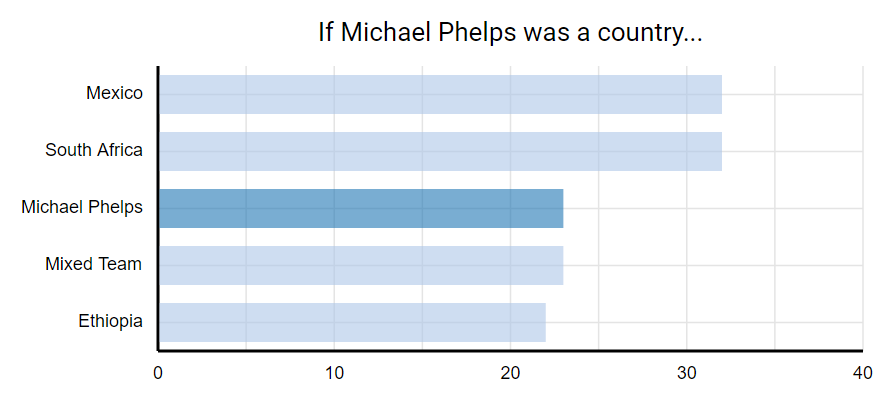
\includegraphics[width=1\columnwidth]{figures/cases-mp}
  \caption{Exploring Olympic medalists using tabular data type provider}
  \label{fig:cases-mp}
\end{subfigure}
\hfill
\begin{subfigure}[b]{0.49\textwidth}
  \centering
  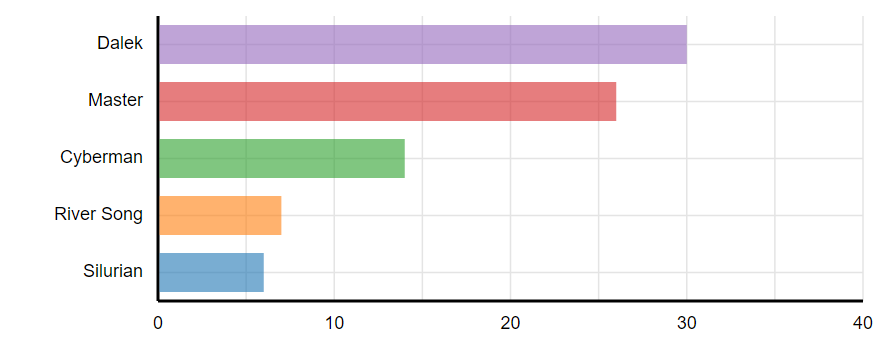
\includegraphics[width=1\columnwidth]{figures/cases-dr}
  \caption{Exploring Dr Who graph database by composing type providers}
  \label{fig:cases-dr}
\end{subfigure}
\vspace{-0.5em}
\caption{Charts produced by two case studies of using The Gamma.}
\label{fig:cases}
\end{figure}

% ==================================================================================================

\section{Case Studies}
\label{sec:cases}

The Gamma aims to simplify programmatic data exploration while keeping enough expressive power
to allow users to create interesting data visualizations. We consider the expressive power in
this section and assess simplicity in the next one. We used The Gamma to analyse
the UK government expenditure, activities of a research institute, Olympic medals and
information about the Doctor Who series\footnote{The analyses are available (non-anonymously)
at \url{http://gallery.thegamma.net}, \url{http://turing.thegamma.net} and \url{http://rio2016.thegamma.net}}.
In this section, we consider two interesting larger examples\footnote{Available
(non-anonymously) at: \url{http://gallery.thegamma.net/86/} and  \url{http://gallery.thegamma.net/87/}, respectively.}.

\subsubsection*{If Michael Phelps were a Country}
Michael Phelps has won so many medals that media compared the number to
countries.\footnote{e.g.~``If Michael Phelps Were A Country, Where Would His Gold Medal Tally Rank?''
 \url{https://www.npr.org/sections/thetorch/2016/08/14/489832779/}}
Media illustrated the story with a chart showing a country league table including Michael Phelps.
We reproduce the chart, shown in Figure~\ref{fig:cases-mp}, using the tabular data type provider:

\begin{thegamma}
\kvd{let} data = olympics.'group data'.'by Team'.'sum Gold'.then
    .'sort data'.'by Gold descending'.then
    .paging.skip(43).take(4).'get series'.'with key Team'.'and value Gold'

\kvd{let} phelps = olympics.'filter data'.'Athlete is'.'Michael Phelps'.then
  .'group data'.'by Athlete'.'sum Gold'.then
  .'get series'.'with key Athlete'.'and value Gold'

charts.bar(data.append(phelps)).setColors(["#aec7e8","#aec7e8","#1f77b4"])
\end{thegamma}

\noindent
The data analysis is done in two commands. The first counts gold medals by countries
and uses paging to fetch 4 countries with suitable number of medals. In the second, we abuse the
grouping operation to aggregate data for just a single group. The two data series are then assigned
to local variables (for readability) and passed to the \ikvd{chart.columns} function.
The case study illustrates when more advanced language features are necessary. The data exploration
itself has been completed via iterative prompting, but producing the final chart currently requires
some manual programming. In practice, this would likely be done with the help of an expert
or by copying code from an example.

\subsubsection*{The Most Frequent Doctor Who Villains}
In the second case study, use a graph database on the Dr Who series and list Dr Who villains
by the number of episodes in which they appear. This case study is interesting as it
combines the graph database provider for fetching the data with the tabular data provider for
summarization:

\begin{thegamma}
drWho.Character.Doctor.'ENEMY OF'.'[any]'.'APPEARED IN'.'[any]'.explore
  .'group data'.'by Character name'.'count distinct Episode name'.then
  .'sort data'.'by Episode name descending'.then
  .paging.take(8).'get series'.'with key Character name'.'and value Episode name'
\end{thegamma}

\noindent
Line 1 use the graph database provider to find all paths linking the Doctor node with any
character linked via \ikvd{ENEMY OF}, followed by any episode linked by \ikvd{APPEARED IN}.
This produces a table that can be analysed using the tabular data provider by choosing the
\ikvd{explore} member. For each character (the villain) we count the total number of
distinct episodes in the table. The result is shown in Figure~\ref{fig:cases-dr}.
The example performs a fairly sophisticated data analysis that involves a graph database query
followed by an SQL-like data aggregation. The code can be fully constructed using iterative
prompting (with the exception of the numbers in paging). Another important feature is that
instantaneous previews support the user during the construction, showing the intermediate result
at each step of the construction.

% ==================================================================================================

% TODO Study improvements
% - The questionaire needs a bit more introduction when you present  the study.
% - When looking at the data for the questionaire, it seems somewhat inconclusive
%    as all the values lie around 2.5.  I think this warrants a bit more discussion.
% - Connected to this, I would recommend to highlight the successes of the study a bit more in the
%     discussion and  presentation of the results. You actually got non-programmers to do
%     sophisticated queries! That you didn't get support for all RQs is perhaps more a result of being quite  ambitious!


\section{User Study}
\label{sec:study}

Our goal was to develop an easy-to-learn tool that non-programmers can use
for producing transparent data analyses. To evaluate the extent to which The Gamma achieves this,
we conducted a user study. We recruited participants among the operations and business team of a
non-profit research organization and investigate three research questions.

\vspace{0.5em}\noindent\emph{RQ1: Can non-programmers use The Gamma?}\hspace{0.3em}
Our first hypothesis is that non-programmers will be able to use The Gamma to explore data. To test
this, we gave participants one of four simple data exploration tasks and assess whether they were
able to complete the task, as well as how much assistance, if any, they needed.

\vspace{0.5em}\noindent\emph{RQ2: Can knowledge transfer between data sources?}\hspace{0.3em}
Our second hypothesis is that users familiar with the iterative prompting principle will be able to
use an unfamiliar data source. We designed two of the four tasks to test this. Participants were
shown a demo using one data source and then asked to complete a task using a different one.

\vspace{0.5em}\noindent\emph{RQ3: Can users learn from just code samples?}\hspace{0.3em}
Our third hypothesis is that users can learn through percolation, i.e.~by looking at the source
code of published analyses. In one of our tasks, participants were given a minimal explanation
of The Gamma (showing how to initiate the iterative prompting process) together with
an extensive code sample.

\subsection{Study Design}
We performed a between-subjects study to evaluate the first experience of using The Gamma.
We recruited 13 participants (5 male, 8 female) from a business team
of a research lab working in non-technical roles (project management,
partnerships, communications) including one former journalist. Only one participant (\#12)
had prior programming experience. We split participants into 4 groups. We gave participants a
brief overview of The Gamma (with content depending on the task) and then asked participants
to complete a task. The four tasks were:

\begin{itemize}
\item \emph{Expenditure.} Participants were given a demo using \emph{worldbank}.
  They were asked to use the \emph{expenditure} data source to compare the UK government spending
  on ``Public order and safety'' and ``Defence'' in terms of GDP.
\item \emph{Lords.} Participants were given a demo using \emph{worldbank}.
  They were asked to use the \emph{lords} data source (a table with House of Lords
  members expenses) to find a members representing London with the highest travel costs.
\item \emph{Worldbank.} Participants were given a minimal demo of iterative prompting and
  a code sample using \emph{worldbank}. They were asked to solve a different task using
  the \emph{worldbank} data source.
\item \emph{Olympics.} Participnts were given a demo using \emph{olympics}.
  They were asked to solve a more complex problem, involving grouping and aggregation,
  using the same data source.
\end{itemize}

\noindent
We let participants work independently, but offered guidance if they got stuck.
Tasks \emph{expenditure} and \emph{lords} aim to answer the questions RQ1 and RQ2; the task
\emph{worldbank} aims to answer RQ1 and RQ3. In \emph{olympics}, we test RQ1 using a more complex
data source and we ask further questions to explore the understanding of the data source. Following the
experiment, we conducted a short semi-structured group interview and later sent participants a follow-up
questionnaire.

\begin{figure}
  \begin{subfigure}[b]{0.49\textwidth}
    \centering
    \begin{tabular}{l l l c l}
      \toprule
        & {\small \textit{Task}}
        & {\small \textit{Kind}} & {\small \textit{Done}}
        & {\small \textit{Notes}} \\
      \midrule
      \small \#1 & \small expenditure & \small cube & \priority{50} & {\small Obtained one data series}\\
      \small \#2 & \small expenditure & \small cube & \priority{100} & {\small Explored furhter data }\\
      \small \#3 & \small expenditure & \small cube & \priority{100}& {\small Explored further data  }\\
      \small \#4 & \small expenditure & \small cube & \priority{75}& {\small Correct member hint }\\
      \small \#5 & \small expenditure & \small cube & \priority{100}& {\small Explored further data }\\
      \small \#6 & \small worldbank & \small cube & \priority{75} & {\small With general syntax hint }\\
      \small \#7 & \small worldbank & \small cube & \priority{100} & {\small Completed very quickly }\\
      \small \#8 & \small worldbank & \small cube & \priority{100} & {\small Extra time to find data }\\
      \small \#9 & \small lords & \small table & \priority{75} & {\small  Composition issues}\\
      \small \#10 & \small lords & \small table & \priority{100} & {\small Completed very quickly }\\
      \small \#11 & \small lords & \small table & \priority{75} & {\small Hint to avoid operations}\\
      \small \#12 & \small olympics & \small table & \priority{75}  & {\small Hint to avoid operations}\\
      \small \#13 & \small olympics & \small table & \priority{75}  & {\small Two operations hints}\\
      \bottomrule
    \end{tabular}
    \caption{Work completed by individual participants; \priorityc{100} = completed,
      \priorityc{75} = required some guidance, \priorityc{50} = partially completed}
    \label{tab:tasks}
  \end{subfigure}
  \hfill
  \begin{subfigure}[b]{0.49\textwidth}
    \centering
    \begin{tabular}{p{17.25em} c c}
      \toprule
        {\small \textit{Questionnaire item}} & {\small \textit{Avg}} & {\small \textit{Sdv}} \\
      \midrule
      \small Considering your experience and possible use of The Gamma in the context of data journalism:\\
      \small \quad I found the system easy to use. & \small 4.00 & \small 0.89\\
      \small \quad Journalists will be able to use it to analyse data. & \small 3.45 & \small 1.04\\
      \small \quad Readers will be able to examine the analyses. & \small 3.73 & \small 0.79\\
      \small Thinking about the usability of the system:\\
      \small \quad Resulting programs are easy to understand. & \small 3.73 & \small 0.79\\
      \small \quad Text editor for creating them was easy to use. & \small 3.73 & \small 0.90\\
      \small \quad Finding items in the auto-complete was easy. & \small 3.45 & \small 1.37\\
      \small I would know how to explore a new data source\\
      \small \quad If given a comprehensive video tutorial. & \small 4.00 & \small 1.26\\
      \small \quad If given a number of code samples. & \small 3.36 & \small 1.12\\
      \small \quad Without any further guidance. & \small 2.45 & \small 1.13 \vspace{0.1em}\\
      \bottomrule
    \end{tabular}
    \caption{Follow-up questionnaire responses using
      a 5-point Likert scale (1 = strongly disagree, 5 = strongly agree) over 11 subjects.}
    \label{tab:quest}
  \end{subfigure}
  \vspace{-0.5em}
  \caption{Summary of the work completed by individual participants and responses to the follow-up questionnaire.}
  \label{tab:tabs}
  \vspace{-0.25em}
\end{figure}

\subsection{Study Results}
Figure~\ref{tab:tabs} shows the results of the study. Most notably, all participants were able to
complete, at least partially, a non-trivial data exploration task and only half of them required
further guidance. Table~\ref{tab:tasks} summarizes the work done by the study participants.
For each participant, we record the task, the kind of data source used in the task and the
level of completion. For participants who needed assistance, the notes section details the help
given. We discuss possible design improvements based on the experience in Section~\ref{sec:study-obs}.

The follow-up questionnaire was sent to all participants a week after the experiment. It was
completed all but two participants (\#8 and \#12). We asked general questions about the usability
of the system together with questions about learning designed to answer RQ2 and RQ3. A summary
of the answers is shown in Table~\ref{tab:quest}.

\subsection*{RQ1: Can non-programmers explore data with The Gamma?}
Three facts allow us to answer RQ1 in the affirmative. First, 9 out of 11 participants agree or
strongly agree that they ``found the system easy to use''. Second, participants spent 10--25 minutes
(average 17 minutes) working with The Gamma and 12 out of 13 completed the task; 6 required assistance,
but 3 of those faced one issue (discussed later) that could be addressed in the introduction.
Third, a number of participants shared positive comments in the interviews.
Participant \#3 found the system simple, but also points out an issue about data provenance,
which we revisit later:

\begin{quote}
\emph{``This is actually pretty simple to use. You think about the logic of what you're actually
  asking and then you try to get it into the format you can. But knowing where it comes from
  would tell you how to trust it.''}
\end{quote}

\noindent
Similarly, participant \#2, notes that The Gamma alleviated their unease about code:

\begin{quote}
\emph{``For somebody who does not do coding or programming, this does not feel that daunting.
  It's not like you're giving me large screen full of code, which is reassurring.''}
\end{quote}

\noindent
Finally, participant \#5 suggested the system could be used as an educational tool for teaching
critical thinking with data. They answer a follow-up question about what training materials would
the students need as follows:

\begin{quote}
\emph{``I don't think they'd need more than 5 minute video (..) this is the data
  source, this is what's in there.''}
\end{quote}

\subsection*{RQ2: Can knowledge transfer between data sources?}
Our study does not conclusively answer RQ2. There is some evidence in favor of a positive answer.
In the practical part, two of the tasks (\emph{expenditure} and \emph{lords}) used a different data
source in the introductory presentation than the one that the participants were asked to explore.
Participants were able to complete those tasks, although \emph{lords} has been more challenging
as it involves a more complex data source. In the interview, participant \#2 also gives a positive
answer:

\begin{quote}
\emph{``I found it quite easy to translate what you showed us in the demo to the new dataset.
   I thought it was quite easy to just get how that works.''}
\end{quote}

\noindent
Negative evidence is offered by the follow-up questionnaire. When asked
whether they would know how to approach a task using a new data source, 6 out of 11 participants
disagree or strongly disagree that they would know how to approach it without any further guidance.
The nature of RQ2 makes it a more challenging question to study and so finding a conclusive answer
arguably requires further research.

\subsection*{RQ3: Can users learn from just code samples?}
A positive answer to RQ3 is supported by the \emph{worldbank} task results, the follow-up questionnaire
and interview comments. In the task, participants were given only a
minimal demo of the iterative prompting principle together with print-out of 2 code samples.
All three were able to complete a related task using the same data source. In the follow-up
questionnaire, only 2 out of 11 participants disagree or strongly disagree that
they would know how to approach a task using an unfamiliar data source when given ``a number
of code samples''.

In the semi-structured interview, participants were asked what would be the most useful format
of educational material about The Gamma (code samples, video tutorials, etc.).
Participant \#7 noted that \emph{``a video would just be this [i.e.~a code sample] anyway''}, while
participant \#13 (former journalist) answered:

\begin{quote}
  \emph{``I think providing one video of one example is good and maybe a couple of little examples
  of code where people can see the kind of things you can do.''}
\end{quote}

\noindent
This is aligned with our design goal. Once the user understands the iterative prompting principle
(which can be done through a video tutorial), they can learn how to use any specific data source
just from code samples.

\subsection{Further Observations}
\label{sec:study-obs}
In this section, we briefly discuss a number of observations about The Gamma design that
emerged from the experiments and follow-up interviews, some of which suggest ways of improving the system.

\subsubsection*{Making Complex Things Possible May Hurt}
The Gamma supports operations such as \ikvd{take(5)}. Most type
providers never generate those, but the provider for working with tabular data is an exception.
When filtering data, the provider allows specifying a condition on numerical attributes such as
\ikvd{olympics.\textquotesingle filter data\textquotesingle.\textquotesingle Year is greater than\textquotesingle(2004)}.

Three participants (\#11, \#12, \#13) struggled to complete a task, because they
initially attempted to use those operations. They violate the iterative prompting
principle as one cannot type `.' after \ikvd{\textquotesingle Year is greater than\textquotesingle}.
This suggests that we should either avoid such operations, or hide them under an ``advanced operations''
tab as a caution to novice users.

\subsubsection*{Benefits and Drawbacks of Text}
The Gamma is based on text to aid transparency. Text implies that there is no hidden state and
the reader sees the full code. The study suggests that using a text editor has both
benefits and drawbacks compared to alternatives such as structured editors~\cite{structure-based,livenut,lamdu}.
Most participants had no difficulty navigating around source code, making edits or deleting code
fragments, which is arguably harder in an unfamiliar structured editor.

On the one hand, we observed two issues in the study. Participant \#2 struggled with correct indentation, starting
a second command with more indentation than needed and participant \#6 had a syntax error in an unrelated command,
which prevents charts from rendering. On the other hand, some participants used the text editor effectively,
e.g.~participant \#5, who used copy-and-paste to fetch the same data series for multiple countries.


\subsubsection*{Understanding the `then' Member}
We asked participants who worked with tabular data about their understanding of the \ikvd{then} member.
This is a regular member (not a keyword), but it has a special meaning in the domain specific language.
Consider the calculation of average travel costs and number of representatives per county in the House of Lords:

\begin{thegamma}
expneses.'group data'.'by County'.'average Travel Costs'.'count distinct Name'.then
\end{thegamma}

\noindent
The \ikvd{then} member is used to complete a part of a query where the user repeatedly
add items to build a list. Here, we select two aggregations to be calculated for each
county before choosing \ikvd{then} and applying other operations such as sorting.
Two participants (\#12 and \#13) thought that \ikvd{then} is used to split a command
over multiple lines, but rejected the idea after experimenting and noting that they can insert
line breaks elsewhere. One correctly concluded that it ``allows us to chain together the
operations'' of the query. Following a hint, participant \#13 reflected:

\begin{quote}
  \emph{``When you explained about the `dot then' that was a really useful thing to know.
  When I found that, I was like this is fine, this is doable. If I knew this from the start,
  it would [have been easier].''}
\end{quote}

\noindent
This comment summarizes an important fact. Although iterative prompting allows the users to start
exploring new data sources, the domain specific languages used by more complex data sources have
their own design principles that users need to understand to use the data source effectively.

% ==================================================================================================

\section{Discussion}
We examine an unexplored point in the design space of tools for data exploration. The Gamma is a
text-based programming environment, but targets non-programmers such as data journalists. We
conclude with a more general discussion of evaluation of the system and the possible applicability
of The Gamma in data journalism.

\subsection{Evaluating Exploratory Research}
The research presented in this paper is qualitative and exploratory in nature. In particular,
we do not make any quantitative claims about the usability of The Gamma and its learning curve.
Our investigation focused on the core iterative prompting principle, but some our case studies
also required using features such as operations with parameters.

Although The Gamma is open-source, it has not been deployed in production in a newsroom so far.
This would lead to valuable insights, but it requires finding a suitable fortuitous opportunity.
Finally, we also do not compare the usability of The Gamma with other popular systems
such as Tableau \cite{tableau}. It would be possible to set tasks that can be completed
in both systems, but the systems have very different aims making such comparison problematic.

\subsection{Evaluating Complex Systems}
Data exploration environments are complex systems that do not yield to simple controlled
experimentation. Olsen~\cite{evaluating} proposes criteria for judging whether a system advances
the state of the art. A number of those apply to The Gamma:

\begin{itemize}
\item \emph{Importance.} Data journalism can make factual claims backed by data more commonplace
and enable wider audience to engage with such claims. As such, we contribute towards
solving an important societal issue.

\item \emph{Expressive leverage.} Iterative prompting stratifies the complexity of data exploration
such that different data sources are accessed through the same unified iterative prompting
interaction principle.

\item \emph{Empowering new participants.} As demonstrated by our user study, The Gamma allows
non-experts, including those not comfortable with code, to perform basic programmatic
data exploration tasks.

\item \emph{Generality.} The Gamma can be used to query data from a wide range of data
sources including tabular data, data cubes and graph databases. The range of possible tasks is
illustrated by case studies presented earlier.
\end{itemize}

\subsection{Applications to Data Journalism}
Although The Gamma targets a broad audience of non-programmers, some of our work has been
particularly motivated by the use of data in journalism. The Gamma is aligned with recent challenges
faced by journalists in that it can help build trust through transparency as well as provide
meaningful ways of reader engagement.

Our study shows that non-experts with background similar
to journalists are able to solve basic data exploration tasks using The Gamma. When asked whether
The Gamma is something that journalists could learn how to use, a former journalist who
participated in our study (\#13) answered:

\begin{quote}
\emph{``Yeah, I think so. There's a lot of effort going into data journalism that
  programming could make much quicker, but I was always nervous about code. (...)
  Something like this would really simplify things.''}
\end{quote}

\noindent
The answer suggests that iterative prompting, does indeed, lower the barrier to entry. Although it
does not fully eliminate complexity involved in data querying, it provides a way of stratifying
it. Iterative prompting makes it easy to get started with data exploration, addressing the initial
``nervousness about code''. By making the source code of data anlyses visible, The Gamma then
enables further learning through percolation.

\subsection{Further Design Issues}
There remain a number of aspects of data exploration in the context of journalism that
The Gamma does not address. Two of those, data provenance and data availability were also
observed by the participants in our study.

\subsubsection*{Data provenance}
Data sources such as \ikvd{olympics} or \ikvd{worldbank} are defined when initializing The Gamma,
but the system does not currently show where such data comes from.
For some tabular data sources, the source is a CSV file published, e.g.~by the government. In this case,
we can easily show the source URL. However, other type providers may pre-process data. Displaying
data source in such cases would require more sophisticated provenance tracking \cite{provenance}.

\subsubsection*{Data availability}
In the current version, The Gamma does not have a way of informing the user what data sources
are available. In other words, the user needs to know the first identifier, such as \ikvd{olympics},
to get started. We could address this by choosing a data source as the first step of iterative
prompting and perhaps typing \ikvd{.olympics}. However, a more fundamental issue is finding
the data source in the first place. This could be partly addressed by a type provider for a
currated online database such as Enigma Public\footnote{\url{https://docs.enigma.com/public}}.
Providing access to open government data repositories such as \url{http://data.gov} and
\url{http://data.gov.uk} is more appealing, but challenging due to their unstructured nature.

\section{Conclusions}
Exploring data in a programming environment that makes the full source code available increases
transparency, reproducibility and empowers users to ask critical questions about the data anlysis.
But can we make those features accessible to non-programmers? In this paper, we presented The Gamma,
a simple data exploration environment for non-programmers that answers this question in the
affirmative.

The Gamma is based on a single interaction principle, \emph{iterative prompting}. It can be used to
complete a range of data exploration tasks using tabular data, data cubes and graph databases.
The design lowers the barrier to entry for programmatic data exploration and makes it easy to learn
the system independently through examples and by experimentation. We implemented The Gamma, make it
available as open source and conducted a user study, which lets us conclude that
The Gamma can be used by non-programmers to construct non-trivial data exploration scripts.

\bibliographystyle{ACM-Reference-Format}
\bibliography{paper}

\end{document}
